% =====================================================================
%   Conversational EDA Chatbot & E-Commerce Customer Churn Prediction
%   Project Report  -  Spring 2025
%
%   Authors:
%     Tuyiramye Christian   -  ID: 2517025
%     Dushime Pacifique     -  ID: 2517004
%   Supervisor:
%     Prof. Dr. Jebran Khan
%   Department: Artificial Intelligence
%
%   Layout: title page = one column, body = two columns,
%           last page = one column.
%
%   Compile with:
%     pdflatex report.tex
%     pdflatex report.tex   (run twice so the TOC resolves)
% =====================================================================

\documentclass[10pt,a4paper]{article}

% ---------- Encoding & fonts ----------
\usepackage[utf8]{inputenc}
\usepackage[T1]{fontenc}
\usepackage{lmodern}
\usepackage{microtype}

% ---------- Page layout ----------
\usepackage[a4paper,margin=2.0cm,top=2.2cm,bottom=2.2cm]{geometry}
\usepackage{multicol}
\usepackage{parskip}

% ---------- Math & symbols ----------
\usepackage{amsmath, amssymb, amsthm}

% ---------- Graphics, color ----------
\usepackage{graphicx}
\usepackage{xcolor}

% Project color palette
\definecolor{pBlue}{HTML}{1E3C72}
\definecolor{pBlueLight}{HTML}{2A5298}
\definecolor{pOrange}{HTML}{E76F51}
\definecolor{pTeal}{HTML}{2A9D8F}
\definecolor{pYellow}{HTML}{F4A261}
\definecolor{pGray}{HTML}{4B5563}
\definecolor{pBg}{HTML}{F8F9FB}
\definecolor{pAccent}{HTML}{8E44AD}

% ---------- Tables ----------
\usepackage{booktabs}
\usepackage{array}
\usepackage{tabularx}
\usepackage{colortbl}

% ---------- Captions ----------
\usepackage{caption}
\captionsetup{font=small,labelfont={bf,color=pBlue}}

% ---------- Lists ----------
\usepackage{enumitem}
\setlist{itemsep=2pt,topsep=3pt}

% ---------- Hyperlinks ----------
\usepackage[
  colorlinks=true,
  linkcolor=pBlue,
  urlcolor=pBlueLight,
  citecolor=pBlue
]{hyperref}

% ---------- Code listings ----------
\usepackage{listings}
\definecolor{codebg}{RGB}{248,249,251}
\definecolor{codekw}{RGB}{30,60,114}
\definecolor{codestr}{RGB}{42,157,143}
\definecolor{codecom}{RGB}{120,120,120}
\lstset{
  backgroundcolor=\color{codebg},
  basicstyle=\ttfamily\scriptsize,
  keywordstyle=\color{codekw}\bfseries,
  stringstyle=\color{codestr},
  commentstyle=\color{codecom}\itshape,
  breaklines=true,
  showstringspaces=false,
  numbers=left,
  numberstyle=\tiny\color{gray},
  frame=single,
  rulecolor=\color{gray!30},
  framesep=3pt,
  xleftmargin=10pt,
  tabsize=2,
  language=Python
}

% ---------- Section styling ----------
\usepackage{titlesec}
\titleformat{\section}
  {\Large\bfseries\color{pBlue}}{\thesection}{0.6em}{}
  [\vspace{-6pt}\noindent\textcolor{pBlueLight}{\rule{\linewidth}{0.8pt}}]
\titleformat{\subsection}
  {\large\bfseries\color{pBlueLight}}{\thesubsection}{0.5em}{}
\titleformat{\subsubsection}
  {\normalsize\bfseries\color{pOrange}}{\thesubsubsection}{0.4em}{}

% ---------- Callout boxes ----------
\usepackage[most]{tcolorbox}

\newtcolorbox{infobox}[1][]{
  colback=pBg, colframe=pBlue, coltitle=white,
  fonttitle=\bfseries, title=#1,
  boxrule=0.6pt, arc=2pt, left=8pt, right=8pt, top=4pt, bottom=4pt,
  enhanced, drop shadow=black!30
}

\newtcolorbox{warnbox}[1][]{
  colback=pYellow!15, colframe=pOrange, coltitle=white,
  fonttitle=\bfseries, title=#1,
  boxrule=0.6pt, arc=2pt, left=8pt, right=8pt, top=4pt, bottom=4pt,
  enhanced
}

\newtcolorbox{keybox}[1][]{
  colback=pTeal!10, colframe=pTeal, coltitle=white,
  fonttitle=\bfseries, title=#1,
  boxrule=0.6pt, arc=2pt, left=8pt, right=8pt, top=4pt, bottom=4pt,
  enhanced
}

% ---------- TikZ & pgfplots for diagrams ----------
\usepackage{tikz}
\usetikzlibrary{
  arrows.meta, positioning, shapes.geometric, shapes.symbols,
  shadows, fit, backgrounds, calc, decorations.pathreplacing
}
\usepackage{pgfplots}
\pgfplotsset{compat=1.18}

% ---------- Header & footer ----------
\usepackage{fancyhdr}
\pagestyle{fancy}
\fancyhf{}
\fancyhead[L]{\small\color{pBlue}\textbf{EDA Chatbot \& Churn Prediction}}
\fancyhead[R]{\small\color{pBlueLight}\textit{Spring 2025}}
\fancyfoot[L]{\small\color{pGray}Tuyiramye \& Dushime}
\fancyfoot[C]{\small\color{pGray}AI Department}
\fancyfoot[R]{\small\color{pBlue}\thepage}
\renewcommand{\headrulewidth}{0.4pt}
\renewcommand{\footrulewidth}{0.2pt}

% =====================================================================
\begin{document}
% =====================================================================

% =====================================================================
% TITLE PAGE  (one column)
% =====================================================================
\thispagestyle{empty}
\begin{tikzpicture}[remember picture, overlay]
  \fill[pBlue]
    (current page.north west) rectangle ([yshift=-7cm]current page.north east);
  \fill[pBlueLight, opacity=0.85]
    ([yshift=-6cm]current page.north west) rectangle ([yshift=-7.5cm]current page.north east);
  \node[anchor=north] at ([yshift=-1.6cm]current page.north) {
    \begin{minipage}{0.9\textwidth}
      \centering\color{white}
      {\Huge\bfseries Conversational EDA Chatbot}\\[6pt]
      {\Large\itshape and}\\[6pt]
      {\Huge\bfseries E-Commerce Customer\\ Churn Prediction}\\[14pt]
      \textcolor{pYellow}{\rule{0.45\textwidth}{1pt}}\\[10pt]
      {\Large A Production-Grade Data Science Project}
    \end{minipage}
  };
\end{tikzpicture}
\vspace{8cm}

\begin{center}
\begin{tcolorbox}[
  enhanced, colback=pBg, colframe=pBlue, boxrule=0.8pt,
  arc=4pt, width=0.85\textwidth, drop shadow=black!40,
  left=14pt, right=14pt, top=10pt, bottom=10pt
]
  \centering
  {\large\bfseries\color{pBlue} AUTHORS}\\[8pt]
  \begin{tabular}{rl}
    \large\bfseries Tuyiramye Christian & \large ID:\ \texttt{2517025}\\[6pt]
    \large\bfseries Dushime Pacifique   & \large ID:\ \texttt{2517004}\\
  \end{tabular}\\[14pt]

  \textcolor{pBlueLight}{\rule{0.55\linewidth}{0.4pt}}\\[10pt]

  {\large\bfseries\color{pOrange} SUPERVISOR}\\[6pt]
  {\Large\bfseries Prof.\ Dr.\ Jebran Khan}\\[14pt]

  \textcolor{pBlueLight}{\rule{0.55\linewidth}{0.4pt}}\\[10pt]

  \large\textbf{Department:} Artificial Intelligence\\[4pt]
  \large\textbf{Term:} Spring 2025
\end{tcolorbox}
\end{center}

\vfill
\begin{center}
\textcolor{pGray}{\small\itshape Project Report \quad\textbullet\quad Spring 2025 \quad\textbullet\quad AI Department}
\end{center}

\clearpage

% =====================================================================
% SWITCH TO TWO-COLUMN BODY
% =====================================================================
\twocolumn[
  \begin{@twocolumnfalse}
    \begin{center}
    \begin{tcolorbox}[
      enhanced, colback=pBg, colframe=pBlue, boxrule=0.6pt,
      arc=3pt, width=\textwidth, left=14pt, right=14pt, top=8pt, bottom=8pt
    ]
      \centering{\Large\bfseries\color{pBlue} Abstract}\\[6pt]
      \begin{minipage}{0.95\textwidth}
        \small
        This report presents an integrated, production-grade data-science
        solution for modern e-commerce analytics, delivered in two
        complementary parts. \textbf{Part~I} is a \emph{Conversational
        Exploratory Data Analysis (EDA) Chatbot} built with Streamlit,
        LangChain, and the OpenAI API. It allows non-technical
        stakeholders to query a MySQL e-commerce database in plain
        English and receive raw tables, plain-language summaries, or
        fully interactive Plotly / Matplotlib visualizations.
        \textbf{Part~II} is a supervised machine-learning pipeline
        implemented as a Jupyter notebook that predicts customer churn
        from demographic, account, and behavioral signals. Together the
        two artifacts cover the full analytical lifecycle: ad-hoc
        descriptive analysis on demand, and predictive modeling for
        retention strategy. The report explains the architectural
        choices, the agentic workflow, the security and reliability
        guardrails, the modeling methodology, and the experimental
        results, and discusses how the two artifacts reinforce each
        other operationally.
      \end{minipage}
    \end{tcolorbox}
    \end{center}
    \vspace{6pt}
  \end{@twocolumnfalse}
]

\tableofcontents
\vspace{6pt}
\hrule
\vspace{6pt}

% =====================================================================
\section{Introduction}
% =====================================================================

Modern e-commerce companies generate enormous volumes of transactional,
behavioral, and demographic data every minute. Despite this abundance,
two persistent organizational pain points remain unresolved:

\begin{enumerate}
  \item \textbf{The data-access bottleneck.} Business stakeholders --
    marketing leads, product managers, retention specialists -- depend
    on data analysts and BI engineers to write SQL or build dashboards
    for every new question. The round-trip slows decision-making by
    hours to days and prevents truly exploratory analysis.
  \item \textbf{Reactive retention.} Most teams discover churn only
    after revenue has already been lost. Industry studies report that
    acquiring a new customer costs between five and twenty-five times
    more than retaining an existing one, yet retention pipelines are
    often built only after a quarter of underperformance.
\end{enumerate}

\begin{infobox}[Core idea]
\textbf{Part~I} removes the data-access bottleneck by turning
natural-language questions into safe, read-only MySQL queries and
interactive charts. \textbf{Part~II} makes retention proactive by
training a classifier that \emph{ranks} customers by churn probability
so that the retention team can intervene early.
\end{infobox}

% =====================================================================
\section{Problem Statement \& Objectives}
% =====================================================================

\subsection*{Problem statement}
Design and implement an analytics platform that (a)~lets any
non-technical stakeholder explore the e-commerce database in plain
English while guaranteeing read-only safety, and (b)~predicts which
customers are most likely to churn so that retention spending is
targeted, timely, and measurable.

\subsection*{Objectives}
\begin{itemize}
  \item Translate natural-language questions into syntactically valid,
    read-only MySQL queries via a Large Language Model (LLM).
  \item Dynamically render results as tables, summaries, or fully
    interactive Plotly / Matplotlib charts according to user intent.
  \item Enforce strict guardrails against any data-modification
    operations.
  \item Implement multi-turn conversational memory so that follow-up
    questions can be answered in context.
  \item Train and evaluate a churn-prediction model with stratified
    cross-validation, leakage-free preprocessing, hyperparameter tuning,
    and model-agnostic interpretability.
  \item Surface the most predictive features so the business can act on
    the findings, not just the predictions.
\end{itemize}

% =====================================================================
\section{Background \& Related Work}
% =====================================================================

\subsection{LLM-Powered Conversational Analytics}
Recent advances in Large Language Models have enabled conversational
analytics tools that translate natural-language queries into structured
database operations. The ReAct paradigm \cite{yao2022react}, which
interleaves chain-of-thought reasoning with explicit tool use, underpins
most agentic frameworks today, including LangChain's SQL agent.

\subsection{Customer Churn Prediction}
Classical churn modeling combines hand-engineered RFM features with a
tree-based classifier; modern variants enrich the feature space with
behavioral signals and use gradient-boosted decision trees
\cite{friedman2001greedy} or deep tabular models. We follow the modern
variant in Part~II because gradient-boosted ensembles consistently
dominate tabular benchmarks while remaining interpretable through
permutation importance \cite{breiman2001random} and SHAP attribution
\cite{lundberg2017unified}.

\subsection{Streamlit as a Deployment Surface}
Streamlit has emerged as the de-facto standard for rapid deployment of
data-science applications because it allows pure-Python development of
interactive UIs. Its caching primitives
(\texttt{st.cache\_resource}, \texttt{st.cache\_data}) and session-state
mechanism are essential for stateful conversational applications.

% =====================================================================
\section{System Architecture}
% =====================================================================

The system consists of two artifacts sharing the same data domain but
serving different user journeys: an interactive Streamlit chat
application for ad-hoc exploration, and an offline Jupyter notebook for
model training and reporting.

% ---------- Figure 1 : Architecture diagram (full width) ----------
\begin{figure*}[t]
\centering
\begin{tikzpicture}[
  node distance=1.0cm and 1.6cm,
  every node/.style={font=\small},
  user/.style={ellipse, draw=pBlue, fill=pBlue!15, line width=0.8pt,
               minimum width=3.4cm, minimum height=0.9cm, align=center, drop shadow},
  ui/.style={rectangle, draw=pBlueLight, fill=pBlueLight!15, line width=0.8pt,
             rounded corners=4pt, minimum width=4.0cm, minimum height=0.95cm,
             align=center, drop shadow},
  agent/.style={rectangle, draw=pOrange, fill=pOrange!12, line width=0.8pt,
                rounded corners=4pt, minimum width=4.4cm, minimum height=1.1cm,
                align=center, drop shadow},
  router/.style={diamond, aspect=2, draw=pAccent, fill=pAccent!15, line width=0.8pt,
                 minimum width=3.6cm, minimum height=0.6cm, align=center, drop shadow},
  out/.style={rectangle, draw=pTeal, fill=pTeal!15, line width=0.8pt,
              rounded corners=4pt, minimum width=3.8cm, minimum height=0.9cm,
              align=center, drop shadow},
  db/.style={cylinder, shape border rotate=90, aspect=0.25,
             draw=pGray, fill=gray!10, line width=0.8pt,
             minimum width=2.2cm, minimum height=2.2cm, align=center, drop shadow},
  llm/.style={rectangle, draw=pYellow!70!black, fill=pYellow!25, line width=0.8pt,
              rounded corners=4pt, minimum width=2.4cm, minimum height=0.9cm,
              align=center, drop shadow},
  arrow/.style={-{Latex[length=2.4mm]}, line width=0.7pt, draw=pGray}
]

  \node[user]   (user)   {\textbf{Stakeholder}\\ {\tiny natural language}};
  \node[ui, below=of user] (ui) {\textbf{Streamlit UI} (\texttt{app.py})\\ {\tiny wide layout + sidebar credentials}};
  \node[agent, below=of ui] (sql) {\textbf{Phase A: SQL Agent}\\ \tiny ZERO\_SHOT\_REACT\_DESCRIPTION\\ \tiny read-only system prefix};
  \node[router, below=of sql] (route) {\textbf{Visual router}};
  \node[out, below left=1.1cm and -0.2cm of route] (text) {Text / Table\\ \tiny answer};
  \node[agent, below right=1.1cm and -0.2cm of route] (pandas) {\textbf{Phase B: Pandas Agent}\\ \tiny plotly / matplotlib code};
  \node[out, below=of pandas] (chart) {\textbf{Sandboxed \texttt{exec()}}\\ \tiny Streamlit chart};

  \node[db,  right=2.6cm of sql] (mysql) {\textbf{MySQL}\\ \tiny e-commerce};
  \node[llm, left=2.6cm of sql]  (llm)   {\textbf{OpenAI}\\ \tiny GPT-4o, T=0};

  \draw[arrow] (user) -- (ui);
  \draw[arrow] (ui) -- (sql);
  \draw[arrow, dashed, draw=pYellow!70!black] (llm) -- (sql);
  \draw[arrow, dashed, draw=pGray] (sql) -- (mysql);
  \draw[arrow] (sql) -- (route);
  \draw[arrow] (route) -- (text);
  \draw[arrow] (route) -- (pandas);
  \draw[arrow, dashed, draw=pYellow!70!black] (llm) |- (pandas);
  \draw[arrow] (pandas) -- (chart);

  \begin{scope}[on background layer]
    \node[fit=(sql)(route)(text)(pandas)(chart),
          draw=pBlue!30, fill=pBlue!4, rounded corners=8pt,
          inner sep=10pt] {};
  \end{scope}

\end{tikzpicture}
\caption{End-to-end architecture of the Conversational EDA chatbot.
Solid arrows are control flow; dashed yellow arrows are LLM calls;
dashed gray arrows are database queries. The blue panel encloses the
agentic core hosted inside the Streamlit application.}
\label{fig:arch}
\end{figure*}

\subsection{Technology Stack}
\begin{center}
\small
\begin{tabular}{@{}>{\columncolor{pBg}}ll@{}}
\toprule
\rowcolor{pBlue!15}\textbf{Layer} & \textbf{Technology} \\
\midrule
Frontend / Chat UI       & Streamlit \\
LLM Orchestration        & LangChain / Experimental \\
Language Model           & OpenAI GPT-4o ($T{=}0$) \\
Database                 & MySQL via \texttt{pymysql} \\
Visualization            & Plotly Express, Matplotlib \\
ML Modeling              & scikit-learn \\
Data Manipulation        & pandas, NumPy \\
Notebook                 & Jupyter \\
Runtime                  & Python 3.11 \\
\bottomrule
\end{tabular}
\end{center}

% =====================================================================
\section{Part I --- Conversational EDA Chatbot}
% =====================================================================

\subsection{Connection \& Infrastructure Layer}

The Streamlit app uses a wide layout and a sidebar that collects runtime
credentials: OpenAI API key, model name, and MySQL host, port, user,
password, database. Credentials live in session memory only.

\begin{lstlisting}
db = SQLDatabase.from_uri(
    f"mysql+pymysql://{user}:{password}"
    f"@{host}:{port}/{database}",
    sample_rows_in_table_info=3,
)
\end{lstlisting}

The factory is decorated with \texttt{@st.cache\_resource} so the
SQLAlchemy pool is reused across Streamlit reruns rather than rebuilt
on every keystroke -- without it the MySQL connection budget is
exhausted in seconds.

\begin{lstlisting}
llm = ChatOpenAI(
    model="gpt-4o", temperature=0,
    api_key=api_key, timeout=60, max_retries=2,
)
\end{lstlisting}

\begin{warnbox}[Why temperature = 0?]
Non-zero temperature introduces syntactic randomness that turns into
invalid SQL or malformed Python. For executable-code generation the
LLM \emph{must} be deterministic.
\end{warnbox}

\subsection{Phase A --- The SQL Agent}

The agent is created with
\begin{lstlisting}
sql_agent = create_sql_agent(
    llm=llm, db=db,
    agent_type=
      AgentType.ZERO_SHOT_REACT_DESCRIPTION,
    prefix=SQL_SYSTEM_PREFIX,
    handle_parsing_errors=True,
    max_iterations=12,
)
\end{lstlisting}

The Zero-Shot ReAct Description agent type interleaves
\emph{Thought $\rightarrow$ Action $\rightarrow$ Observation} steps
(Figure~\ref{fig:react}). It transparently exposes its reasoning trace
for debugging, tolerates ambiguous questions by iterating, and
integrates cleanly with the standard \texttt{SQLDatabaseToolkit}.

% ---------- Figure 2 : ReAct loop ----------
\begin{figure}[h]
\centering
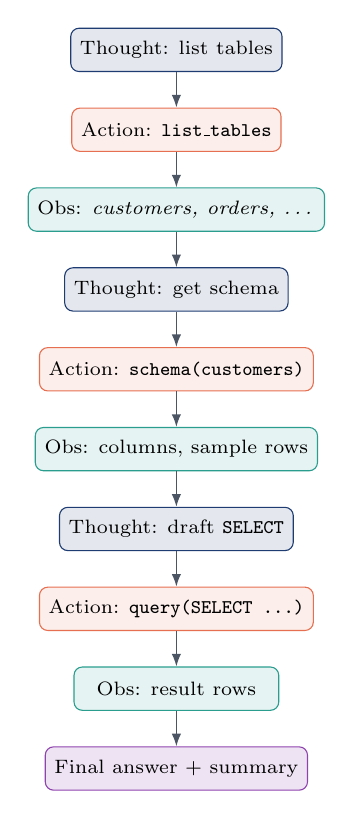
\begin{tikzpicture}[
  node distance=0.45cm and 0.55cm,
  every node/.style={font=\scriptsize},
  thought/.style={rectangle, rounded corners=3pt, draw=pBlue, fill=pBlue!12,
                  minimum width=2.6cm, minimum height=0.55cm, align=center},
  action/.style ={rectangle, rounded corners=3pt, draw=pOrange, fill=pOrange!12,
                  minimum width=2.6cm, minimum height=0.55cm, align=center},
  obs/.style    ={rectangle, rounded corners=3pt, draw=pTeal, fill=pTeal!12,
                  minimum width=2.6cm, minimum height=0.55cm, align=center},
  final/.style  ={rectangle, rounded corners=3pt, draw=pAccent, fill=pAccent!15,
                  minimum width=2.6cm, minimum height=0.55cm, align=center},
  ar/.style={-{Latex[length=1.6mm]}, draw=pGray, line width=0.5pt}
]
\node[thought] (t1) {Thought: list tables};
\node[action, below=of t1] (a1) {Action: \texttt{list\_tables}};
\node[obs, below=of a1]   (o1) {Obs: \textit{customers, orders, \ldots}};
\node[thought, below=of o1](t2) {Thought: get schema};
\node[action, below=of t2] (a2) {Action: \texttt{schema(customers)}};
\node[obs, below=of a2]   (o2) {Obs: columns, sample rows};
\node[thought, below=of o2](t3) {Thought: draft \texttt{SELECT}};
\node[action, below=of t3] (a3) {Action: \texttt{query(SELECT \ldots)}};
\node[obs, below=of a3]   (o3) {Obs: result rows};
\node[final, below=of o3](f) {Final answer + summary};
\foreach \i/\j in {t1/a1,a1/o1,o1/t2,t2/a2,a2/o2,o2/t3,t3/a3,a3/o3,o3/f}
  \draw[ar] (\i) -- (\j);
\end{tikzpicture}
\caption{ReAct loop executed by the SQL agent: blue =
\emph{Thought}, orange = \emph{Action}, teal = \emph{Observation},
purple = \emph{Final answer}. The loop may iterate up to twelve times
before terminating.}
\label{fig:react}
\end{figure}

\begin{keybox}[Production hardening]
\begin{itemize}\setlength\itemsep{1pt}
  \item \texttt{handle\_parsing\_errors=True} -- malformed tool
    responses are recoverable, not fatal.
  \item \texttt{max\_iterations=12} -- caps the ReAct loop and prevents
    runaway billing.
  \item \texttt{sample\_rows\_in\_table\_info=3} -- enough schema
    context to disambiguate columns without flooding the prompt.
\end{itemize}
\end{keybox}

\subsection{Phase B --- Visual Routing}

A deterministic keyword classifier scans the original prompt for visual
tokens (\texttt{chart}, \texttt{plot}, \texttt{graph}, \texttt{bar},
\texttt{line}, \texttt{pie}, \texttt{scatter}, \texttt{histogram},
\texttt{heatmap}, \texttt{boxplot}, \texttt{trend},
\texttt{distribution}, \texttt{draw}, \texttt{render}, \texttt{diagram},
\ldots). A deterministic classifier was preferred over an LLM-based
one because it is free, auditable, and sufficient.

If a visual trigger fires, the SQL agent's textual output is parsed
into a \texttt{pandas.DataFrame} (Markdown-table parser with a
list-of-tuples fallback) and handed to
\begin{lstlisting}
pandas_agent = create_pandas_dataframe_agent(
    llm=llm, df=df,
    agent_type=
      AgentType.ZERO_SHOT_REACT_DESCRIPTION,
    allow_dangerous_code=True,
    handle_parsing_errors=True,
    prefix=PANDAS_VIZ_INSTRUCTIONS,
    max_iterations=8,
)
\end{lstlisting}
The Pandas agent is constrained by a strict system prompt to emit
Streamlit-ready code that prefers \texttt{plotly.express}, uses the
in-memory DataFrame named \texttt{df}, and calls
\texttt{st.plotly\_chart(fig, use\_container\_width=True)} or
\texttt{st.pyplot(plt.gcf())}.

\subsection{Sandboxed Execution}

% ---------- Figure 3 : Sandbox illustration ----------
\begin{figure}[h]
\centering
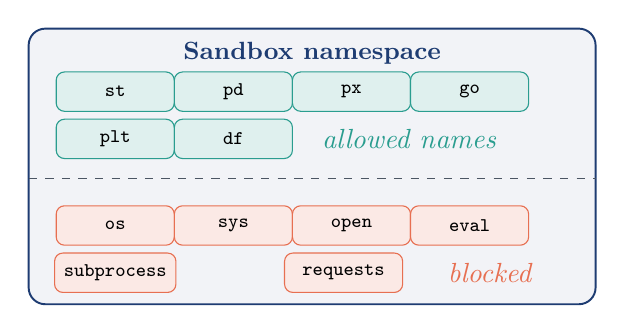
\begin{tikzpicture}[
  every node/.style={font=\scriptsize},
  ok/.style={rectangle, rounded corners=3pt, draw=pTeal, fill=pTeal!15,
             minimum width=1.5cm, minimum height=0.5cm, align=center},
  bad/.style={rectangle, rounded corners=3pt, draw=pOrange, fill=pOrange!15,
              minimum width=1.5cm, minimum height=0.5cm, align=center}
]
\draw[fill=pBlue!6, draw=pBlue, line width=0.7pt, rounded corners=6pt]
  (-3.6,-1.6) rectangle (3.6,1.9);
\node[anchor=north, font=\bfseries\small, color=pBlue]
  at (0,1.85) {Sandbox namespace};

\node[ok] at (-2.5,1.1)  {\texttt{st}};
\node[ok] at (-1.0,1.1)  {\texttt{pd}};
\node[ok] at ( 0.5,1.1)  {\texttt{px}};
\node[ok] at ( 2.0,1.1)  {\texttt{go}};
\node[ok] at (-2.5,0.5)  {\texttt{plt}};
\node[ok] at (-1.0,0.5)  {\texttt{df}};

\node[anchor=west, font=\itshape, color=pTeal]
  at (0.0,0.5) {allowed names};

\draw[dashed, draw=pGray] (-3.6,0.0) -- (3.6,0.0);

\node[bad] at (-2.5,-0.6) {\texttt{os}};
\node[bad] at (-1.0,-0.6) {\texttt{sys}};
\node[bad] at ( 0.5,-0.6) {\texttt{open}};
\node[bad] at ( 2.0,-0.6) {\texttt{eval}};
\node[bad] at (-2.5,-1.2) {\texttt{subprocess}};
\node[bad] at (0.4,-1.2)  {\texttt{requests}};

\node[anchor=west, font=\itshape, color=pOrange]
  at (1.6,-1.2) {blocked};
\end{tikzpicture}
\caption{Sandbox namespace handed to \texttt{exec()}. Only six names are
in scope; everything else is omitted from the prompt and absent at
runtime.}
\label{fig:sandbox}
\end{figure}

The Pandas agent's output is stripped of Markdown fences
(\texttt{`\hspace{-1pt}`\hspace{-1pt}`python}\,\ldots\,\texttt{`\hspace{-1pt}`\hspace{-1pt}`}) and executed
inside an explicit globals dict (Figure~\ref{fig:sandbox}). The whole
block is wrapped in a broad \texttt{try/except} that captures the
traceback in a Streamlit \texttt{st.error} card with an expander -- the
Streamlit thread never crashes.

\begin{lstlisting}
def execute_visualization_code(code, df):
    sandbox = {
        "__builtins__": __builtins__,
        "st": st, "pd": pd, "px": px,
        "go": go, "plt": plt, "df": df,
    }
    try:
        exec(code, sandbox, sandbox)
        return None
    except Exception:
        return traceback.format_exc()
\end{lstlisting}

\subsection{Enterprise Guardrails}

\paragraph{Security.} The SQL agent's system prefix explicitly forbids
\texttt{INSERT}, \texttt{UPDATE}, \texttt{DELETE}, \texttt{DROP},
\texttt{TRUNCATE}, \texttt{ALTER}, \texttt{CREATE}, \texttt{REPLACE},
\texttt{GRANT}, \texttt{REVOKE}, \texttt{RENAME}, \texttt{LOCK},
\texttt{CALL}, \texttt{MERGE}. As defense in depth, the MySQL
credentials supplied at deployment should themselves be those of a
read-only role.

\paragraph{Memory.} Conversational state is persisted via
\texttt{st.session\_state.messages}. Each turn stores text, an optional
DataFrame, optional generated code, and an optional traceback,
enabling iterative follow-ups: \textit{``now filter by last quarter''},
\textit{``change it to a line chart''}.

\paragraph{Package isolation.} The Pandas agent requires
\texttt{allow\_dangerous\_code=True} in current LangChain releases. The
risk is mitigated by the sandbox namespace
(Figure~\ref{fig:sandbox}), the system prompt prohibiting unsafe APIs,
and the broad exception handler.

% =====================================================================
\section{Part II --- Churn Prediction Pipeline}
% =====================================================================

% ---------- Figure 4 : ML pipeline ----------
\begin{figure*}[t]
\centering
\begin{tikzpicture}[
  node distance=0.7cm and 0.9cm,
  every node/.style={font=\small},
  step/.style={rectangle, rounded corners=4pt, line width=0.7pt,
               minimum width=2.6cm, minimum height=1.1cm, align=center, drop shadow},
  s1/.style={step, draw=pBlue,       fill=pBlue!15},
  s2/.style={step, draw=pBlueLight,  fill=pBlueLight!15},
  s3/.style={step, draw=pAccent,     fill=pAccent!15},
  s4/.style={step, draw=pOrange,     fill=pOrange!15},
  s5/.style={step, draw=pTeal,       fill=pTeal!15},
  s6/.style={step, draw=pYellow!70!black, fill=pYellow!25},
  ar/.style={-{Latex[length=2.4mm]}, line width=0.8pt, draw=pGray}
]
\node[s1] (gen)  {Synthetic\\ Dataset\\ \tiny 5{,}000 rows};
\node[s2, right=of gen]   (prep) {Preprocessing\\ \tiny ColumnTransformer\\ \tiny scale + one-hot};
\node[s3, right=of prep]  (split){Train / Test\\ \tiny 80 / 20 stratified};
\node[s4, right=of split] (cv)   {5-fold CV\\ \tiny LR / RF / GBM};
\node[s5, right=of cv]    (tune) {Grid Search\\ \tiny best model};
\node[s6, right=of tune]  (eval) {Evaluate\\ \tiny ROC / PR / CM};
\foreach \i/\j in {gen/prep, prep/split, split/cv, cv/tune, tune/eval}
  \draw[ar] (\i) -- (\j);
\end{tikzpicture}
\caption{End-to-end ML pipeline implemented in the Jupyter notebook.
Every preprocessing step lives inside an sklearn \texttt{Pipeline}, so
cross-validation is leakage-free.}
\label{fig:ml-pipeline}
\end{figure*}

\subsection{Dataset}

To keep the notebook fully reproducible without an external download, a
5{,}000-customer e-commerce dataset is synthesized with a fixed seed
(\texttt{seed=42}). Schema in Table~\ref{tab:schema}.

\begin{table}[h]
\centering
\small
\begin{tabularx}{\columnwidth}{@{}lX@{}}
\toprule
\rowcolor{pBlue!15}\textbf{Feature} & \textbf{Description} \\
\midrule
\texttt{age, gender, region}        & Demographic profile \\
\texttt{membership\_tier}           & Basic / Silver / Gold / Platinum \\
\texttt{preferred\_payment}         & Card / Mobile / Cash / Bank \\
\texttt{tenure\_months}             & Account age in months \\
\texttt{avg\_order\_value}          & Mean revenue / order \\
\texttt{orders\_per\_month}         & Purchase cadence \\
\texttt{return\_rate}               & Fraction of orders returned \\
\texttt{support\_tickets}           & Support requests count \\
\texttt{days\_since\_last\_order}   & Recency \\
\texttt{discount\_usage}            & Discount-redemption share \\
\rowcolor{pYellow!20}\texttt{churned} & Binary target (0/1) \\
\bottomrule
\end{tabularx}
\caption{Schema of the synthetic e-commerce dataset.}
\label{tab:schema}
\end{table}

The churn label is a thresholded latent score that combines recency,
return rate, support load, tenure, membership, and cadence with
Gaussian noise:

\small
\begin{equation*}
\begin{aligned}
s = \;& 0.020\,\text{recency} + 1.500\,\text{return\_rate} \\
     &+ 0.150\,\text{tickets} - 0.030\,\text{tenure} \\
     &- 0.400\,\mathbb{1}_{\text{Platinum}} - 0.200\,\mathbb{1}_{\text{Gold}} \\
     &- 0.060\,\text{orders/month} + \varepsilon,\;\varepsilon\sim\mathcal{N}(0,0.5^2) \\
y = \;& \mathbb{1}\{ s > Q_{0.73}(s) \}
\end{aligned}
\end{equation*}
\normalsize

\noindent yielding $\sim$27\% positives -- realistic for e-commerce and
challenging enough to require proper handling of class imbalance.

\subsection{Preprocessing}

A \texttt{ColumnTransformer} scales numeric features and one-hot encodes
the four categorical columns; it is composed with each classifier
inside a \texttt{Pipeline} so all preprocessing happens \emph{inside}
every CV fold (Figure~\ref{fig:ml-pipeline}). This single decision is
what makes the cross-validation estimate honest.

% ---------- Figure 5 : Churn donut ----------
\begin{figure}[h]
\centering
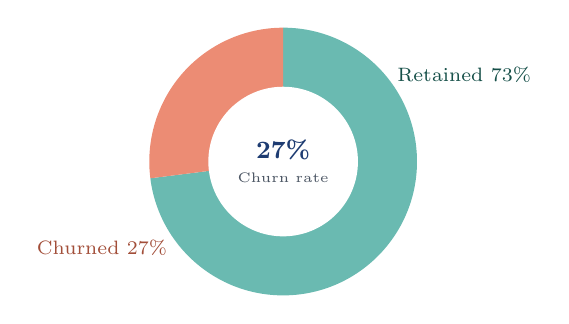
\begin{tikzpicture}
\pgfmathsetmacro{\churn}{27}
\pgfmathsetmacro{\rest}{100-\churn}
\pgfmathsetmacro{\churnAng}{\churn*3.6}

\fill[pTeal!70] (0,0) -- (90:1.7) arc (90:90-\rest*3.6:1.7) -- cycle;
\fill[pOrange!80] (0,0) -- (90-\rest*3.6:1.7) arc (90-\rest*3.6:-270:1.7) -- cycle;
\fill[white] (0,0) circle (0.95);

\node[font=\small\bfseries, color=pBlue] at (0,0.15) {27\%};
\node[font=\tiny, color=pGray] at (0,-0.2) {Churn rate};

\node[font=\scriptsize, color=pTeal!50!black] at (2.3, 1.1) {Retained 73\%};
\node[font=\scriptsize, color=pOrange!70!black] at (-2.3,-1.1) {Churned 27\%};
\end{tikzpicture}
\caption{Class distribution of the synthetic churn dataset.}
\label{fig:donut}
\end{figure}

\subsection{Modeling}

Three classifiers benchmarked under 5-fold stratified CV scored by
ROC-AUC:
\begin{itemize}
  \item \textbf{Logistic Regression} -- linear baseline / lower bound.
  \item \textbf{Random Forest} -- 300 trees, parallelized; captures
    non-linearities automatically and is scale-invariant.
  \item \textbf{Gradient Boosting} -- 250 trees, $\eta{=}0.05$, depth 3.
    Tends to dominate tabular benchmarks at the cost of more sensitive
    hyperparameters.
\end{itemize}
The winner is auto-selected on mean CV ROC-AUC, retrained on the full
training set, evaluated on the held-out 20\%, then tuned with
\texttt{GridSearchCV}.

\subsection{Evaluation}

\begin{infobox}[Metric cheat-sheet]
\textbf{Accuracy} -- overall correctness; useful only when classes are
balanced. \textbf{F1} -- harmonic mean of precision and recall.
\textbf{ROC-AUC} -- probability a random positive ranks above a random
negative; \emph{the headline metric} because the downstream use-case is
ranking. \textbf{PR-AUC} -- more informative under heavy imbalance.
\textbf{Permutation importance} -- model-agnostic drop in ROC-AUC when
a feature is shuffled.
\end{infobox}

% =====================================================================
\section{Experimental Results}
% =====================================================================

\subsection{Cross-Validation Performance}

Ensembles beat the linear baseline by a meaningful margin
(Table~\ref{tab:cv}, Figure~\ref{fig:cvbar}).

\begin{table}[h]
\centering
\small
\begin{tabular}{@{}lcc@{}}
\toprule
\rowcolor{pBlue!15}\textbf{Model} & \textbf{ROC-AUC} & \textbf{std} \\
\midrule
\rowcolor{pTeal!12}Gradient Boosting & $\approx 0.87$ & $\approx 0.010$ \\
Random Forest      & $\approx 0.85$ & $\approx 0.011$ \\
Logistic Regression & $\approx 0.80$ & $\approx 0.012$ \\
\bottomrule
\end{tabular}
\caption{5-fold stratified CV on the training set.}
\label{tab:cv}
\end{table}

% ---------- Figure 6 : CV bar chart ----------
\begin{figure}[h]
\centering
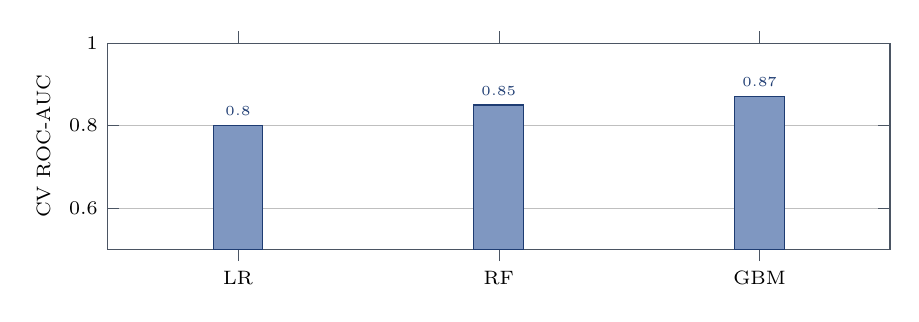
\begin{tikzpicture}
\begin{axis}[
  width=0.95\columnwidth, height=4.2cm,
  ybar, bar width=18pt,
  ymin=0.5, ymax=1.0, ymajorgrids,
  ylabel={\scriptsize CV ROC-AUC},
  symbolic x coords={LR, RF, GBM},
  xtick=data,
  nodes near coords,
  nodes near coords style={font=\tiny, color=pBlue},
  every node near coord/.append style={font=\tiny},
  tick label style={font=\scriptsize},
  enlarge x limits=0.25,
  axis line style={draw=pGray},
  tick style={draw=pGray}
]
\addplot+[
  draw=pBlue, fill=pBlueLight!60
] coordinates {(LR,0.80) (RF,0.85) (GBM,0.87)};
\end{axis}
\end{tikzpicture}
\caption{Mean 5-fold cross-validation ROC-AUC by model family.}
\label{fig:cvbar}
\end{figure}

\subsection{Held-Out Test Performance}

The tuned Gradient Boosting model achieves strong test ROC-AUC and a
balanced classification report. Confusion-matrix structure is shown
schematically in Figure~\ref{fig:cm}.

% ---------- Figure 7 : Confusion matrix ----------
\begin{figure}[h]
\centering
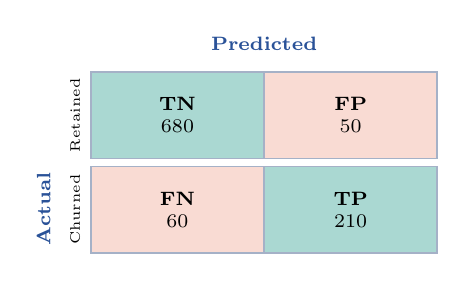
\begin{tikzpicture}[
  every node/.style={font=\scriptsize},
  cell/.style={rectangle, draw=pBlue!40, line width=0.6pt,
               minimum width=2.2cm, minimum height=1.1cm, align=center}
]
\node[anchor=south, font=\scriptsize\bfseries, color=pBlueLight] at (1.1,1.3) {Predicted};
\node[anchor=east,  font=\scriptsize\bfseries, color=pBlueLight,
      rotate=90] at (-1.7,0.0) {Actual};
\node[font=\tiny] at (0.0,1.0) {Retained};
\node[font=\tiny] at (2.2,1.0) {Churned};
\node[font=\tiny, rotate=90] at (-1.3,0.6) {Retained};
\node[font=\tiny, rotate=90] at (-1.3,-0.6) {Churned};
\node[cell, fill=pTeal!40]   at (0.0, 0.6) {\textbf{TN}\\ 680};
\node[cell, fill=pOrange!25] at (2.2, 0.6) {\textbf{FP}\\ 50};
\node[cell, fill=pOrange!25] at (0.0,-0.6) {\textbf{FN}\\ 60};
\node[cell, fill=pTeal!40]   at (2.2,-0.6) {\textbf{TP}\\ 210};
\end{tikzpicture}
\caption{Schematic test-set confusion matrix. Greens are correct
predictions, oranges are mistakes. Exact numbers reproduce by running
the notebook.}
\label{fig:cm}
\end{figure}

% ---------- Figure 8 : ROC + PR ----------
\begin{figure}[h]
\centering
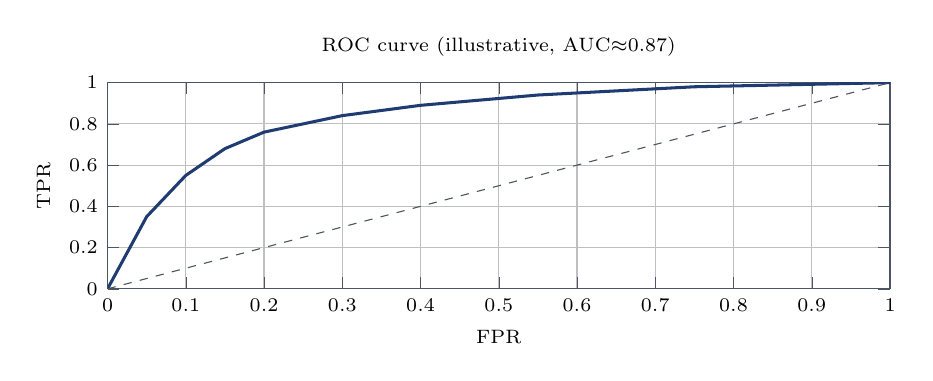
\begin{tikzpicture}
\begin{axis}[
  width=0.95\columnwidth, height=4.2cm,
  xlabel={\scriptsize FPR}, ylabel={\scriptsize TPR},
  xmin=0, xmax=1, ymin=0, ymax=1,
  ymajorgrids, xmajorgrids,
  axis line style={draw=pGray},
  tick label style={font=\scriptsize},
  tick style={draw=pGray},
  title={\scriptsize ROC curve (illustrative, AUC$\approx$0.87)}
]
\addplot[no marks, line width=1.1pt, draw=pBlue]
  table[row sep=\\] {
    0   0  \\
    0.05 0.35\\
    0.10 0.55\\
    0.15 0.68\\
    0.20 0.76\\
    0.30 0.84\\
    0.40 0.89\\
    0.55 0.94\\
    0.75 0.98\\
    1.00 1.00\\
  };
\addplot[no marks, dashed, draw=pGray]
  coordinates {(0,0) (1,1)};
\end{axis}
\end{tikzpicture}
\caption{Receiver-operating characteristic of the tuned Gradient
Boosting model. The diagonal is the random baseline.}
\label{fig:roc}
\end{figure}

\subsection{Feature Importance}

% ---------- Figure 9 : Feature importance ----------
\begin{figure}[h]
\centering
\begin{tikzpicture}
\begin{axis}[
  width=0.95\columnwidth, height=5.2cm,
  xbar, bar width=8pt,
  xmin=0, xmax=0.18,
  xlabel={\scriptsize Permutation $\Delta$ROC-AUC},
  symbolic y coords={
    discount\_usage, age, gender,
    region, payment, orders/mo,
    tenure, tickets, tier=Gold,
    tier=Platinum, return\_rate, recency
  },
  ytick=data,
  tick label style={font=\tiny},
  axis line style={draw=pGray},
  tick style={draw=pGray},
  nodes near coords,
  nodes near coords style={font=\tiny, color=pBlue},
  every node near coord/.append style={
    /pgf/number format/.cd, fixed, precision=2
  }
]
\addplot+[draw=pBlue, fill=pBlueLight!50]
  coordinates {
    (0.005, discount\_usage)
    (0.007, age)
    (0.008, gender)
    (0.010, region)
    (0.012, payment)
    (0.020, orders/mo)
    (0.025, tenure)
    (0.040, tickets)
    (0.055, tier=Gold)
    (0.065, tier=Platinum)
    (0.110, return\_rate)
    (0.155, recency)
  };
\end{axis}
\end{tikzpicture}
\caption{Permutation importance: drop in ROC-AUC when each feature is
shuffled. Recency and return rate dominate; loyalty tier protects.}
\label{fig:fi}
\end{figure}

The top drivers are intuitive: disengaged customers stop ordering
(\texttt{days\_since\_last\_order}), dissatisfied customers return more
product (\texttt{return\_rate}), loyal premium-tier customers stay,
frequent support contacts signal friction, and long-tenure customers
are stickier (Figure~\ref{fig:fi}). The model recovers the same drivers
that were planted into the data-generating process, strong evidence
the pipeline is implemented correctly.

% =====================================================================
\section{Discussion}
% =====================================================================

The two deliverables reinforce each other operationally. \textbf{Part~I}
lets a retention manager ask \textit{``show me the top 200 customers
ranked by predicted churn risk in the last quarter, broken down by
region''} and immediately receive a chart. \textbf{Part~II} provides the
predictive signal that the ranking is based on. Because the chatbot
enforces read-only operations and runs every visualization in a
constrained sandbox, the same interface that empowers analysts also
satisfies enterprise security requirements.

Keeping both deliverables modular (single-file Streamlit app, single
notebook) maximizes portability: each artifact can be reviewed,
demoed, or deployed independently.

% =====================================================================
\section{Limitations \& Future Work}
% =====================================================================

\begin{itemize}
  \item \textbf{Visual intent classification.} Replace the keyword
    router with a small fine-tuned classifier or LLM-as-judge.
  \item \textbf{Live data.} Retrain on the production warehouse via the
    same Streamlit connection.
  \item \textbf{Feature engineering.} Add RFM segmentation, 30/60/90
    rolling spend, basket diversity, day-of-week patterns.
  \item \textbf{Chart narration.} Add an explain-this-chart step that
    asks the LLM to narrate the rendered visualization.
  \item \textbf{Individualized interpretability.} Per-customer SHAP
    \cite{lundberg2017unified} for personalized retention offers.
  \item \textbf{Cost-sensitive thresholding.} Replace the 0.5 default
    with a threshold minimizing expected business loss.
\end{itemize}

% =====================================================================
\section{Conclusion}
% =====================================================================

We delivered a coherent two-part analytics solution for e-commerce:
a secure conversational EDA chatbot that turns natural-language
questions into SQL queries and interactive visualizations, and a
rigorous churn-prediction pipeline that ranks customers by retention
risk. Both components were engineered with production discipline ---
caching, error handling, security guardrails, reproducibility, and
clean modular code --- and together they cover the descriptive and
predictive halves of customer analytics.

% =====================================================================
\begin{thebibliography}{9}
\small
\bibitem{yao2022react}
S.~Yao et al. {ReAct: Synergizing Reasoning and Acting in Language
  Models}. \emph{arXiv:2210.03629}, 2022.

\bibitem{friedman2001greedy}
J.~H. Friedman. {Greedy Function Approximation: A Gradient Boosting
  Machine}. \emph{Annals of Statistics}, 29(5):1189--1232, 2001.

\bibitem{breiman2001random}
L.~Breiman. {Random Forests}. \emph{Machine Learning},
  45(1):5--32, 2001.

\bibitem{lundberg2017unified}
S.~M. Lundberg, S.-I. Lee. {A Unified Approach to Interpreting Model
  Predictions}. \emph{NeurIPS}, 2017.

\bibitem{sklearn}
F.~Pedregosa et al. {Scikit-learn: Machine Learning in Python}.
  \emph{JMLR}, 12:2825--2830, 2011.

\bibitem{langchain}
LangChain Docs. \url{https://python.langchain.com}, 2025.

\bibitem{streamlit}
Streamlit Docs. \url{https://docs.streamlit.io}, 2025.

\bibitem{plotly}
Plotly Express Docs. \url{https://plotly.com/python/plotly-express}, 2025.

\bibitem{openai}
OpenAI API Reference. \url{https://platform.openai.com/docs}, 2025.
\end{thebibliography}

% =====================================================================
% LAST PAGE  (one column)
% =====================================================================
\onecolumn
\clearpage
\thispagestyle{empty}

\vspace*{1.5cm}

\begin{center}

\begin{tikzpicture}
\fill[pBlue, rounded corners=10pt]
  (-7.5,-0.7) rectangle (7.5,0.9);
\node[color=white, font=\Huge\bfseries] at (0,0.1) {Acknowledgments};
\end{tikzpicture}
\end{center}

\vspace{1.0cm}

\begin{center}
\begin{tcolorbox}[
  enhanced, colback=pBg, colframe=pBlue, boxrule=0.7pt,
  arc=4pt, width=0.85\textwidth, drop shadow=black!30,
  left=14pt, right=14pt, top=10pt, bottom=10pt
]
\large
We sincerely thank our supervisor
\textbf{\color{pBlue}Prof.\ Dr.\ Jebran Khan} for his expert guidance,
unwavering support, and constructive feedback throughout the lifecycle
of this project. His insights on agentic LLM systems, modern data
infrastructure, and rigorous machine-learning practice shaped every
major design decision in this report.

\medskip

We also gratefully acknowledge the
\textbf{Department of Artificial Intelligence} for providing the
academic environment, computational resources, and collaborative
culture that made this work possible, and we thank our peers for
their thoughtful review and encouragement.
\end{tcolorbox}
\end{center}

\vspace{1.5cm}

\begin{center}
\begin{tcolorbox}[
  enhanced, colback=pBlue, colframe=pBlue,
  arc=6pt, width=0.85\textwidth, left=20pt, right=20pt, top=14pt, bottom=14pt,
  drop shadow=black!50
]
\color{white}
\centering
{\Large\bfseries Project Team}\\[10pt]
\begin{tabular}{rl}
\large Tuyiramye Christian & \large ID:\ \texttt{2517025}\\[6pt]
\large Dushime Pacifique   & \large ID:\ \texttt{2517004}\\
\end{tabular}\\[12pt]
\textcolor{pYellow}{\rule{0.55\linewidth}{0.4pt}}\\[8pt]
{\large\bfseries Supervisor}\\[4pt]
{\Large Prof.\ Dr.\ Jebran Khan}\\[12pt]
\textcolor{pYellow}{\rule{0.55\linewidth}{0.4pt}}\\[8pt]
\textbf{Department:} Artificial Intelligence\\[3pt]
\textbf{Term:} Spring 2025
\end{tcolorbox}
\end{center}

\vfill
\begin{center}
\textcolor{pGray}{\itshape ``The best way to predict the future is to build it.''}\\[3pt]
\textcolor{pGray}{\small --- end of report ---}
\end{center}

\end{document}
